\documentclass[t,compress=false,usepdftitle=false]{beamer}
%%
\usetheme{LMU}
%%
\usepackage{array}
\usepackage{multicol}
\usepackage{amsmath}
\usepackage{esvect}
%%
\input{commands.tex}
%%
\title[Stencil Interpolation]{Stencil Interpolation for Projected Coordinates}
\author[Baumann and Weism{\"u}ller]{S.~Baumann and J.~Weism{\"u}ller}
\date{Geocomputing, 3.7.2015}
\institute{Geophysics\\Department of Earth- and Environmental Sciences\\Ludwig-Maximilians-Universit{\"a}t M{\"u}nchen}
%%
\graphicspath{{./Pictures/}}
\setcounter{tocdepth}{2}
\beamertemplatenavigationsymbolsempty
\pdfpageattr{/Group << /S /Transparency /I true /CS /DeviceRGB>>}


%
% =============================================================================
%   some customized commands
% =============================================================================
%
%\newtheorem{theorem}{Theorem}
\renewcommand{\div}{\mbox{div}}
\def\RR{\mathbb{R}}
\def\P{\mathcal{P}}

% =============================================================================
\begin{document}
% =============================================================================
%
\frame{\titlepage}
%
% =============================================================================
%   Motivation
% =============================================================================
%
\section{Motivation}
\subsection{Motivation}
%
\begin{frame}\frametitle{Motivation}
%
todo ...
%
\end{frame}

% =============================================================================
%    Results for spherepoisson
% =============================================================================
%
\section{Spherepoisson}
\subsection{Spherepoisson}
%
% =============================================================================
%
\begin{frame}\frametitle{Model Description}
We consider the PDE 
\begin{align*}
\div u &= f\quad \text{in }\Omega \\
     u &= 0\quad \text{on }\partial\Omega
\end{align*}
where $\Omega$ is a spherical shell
\begin{equation*}
\Omega = \left\{(x,y,z) \in\RR^3\quad:\quad 0.546^2 \leq x^2+y^2+z^2 \leq 1\right\}
\end{equation*}
and the right-hand side $f$ is given by
\begin{equation*}
f(x,y,z) = 3\cdot \sin(x)\sin(y)\sin(z).
\end{equation*}
%
\end{frame}
%
% =============================================================================
%
\begin{frame}\frametitle{Discritization}
In the classical HHG approach the spherical shell is approximated
by (at least 60) Tetrahedra (Macro-Tetrahedra).
This input grid is split into primitives of different dimensions 
(Vertices, Edges, Faces and \cempha{Tetrahedra})

\begin{figure}\centering
\includegraphics[width=0.5\textwidth]{macroTet_projected_constant_coords.png}
\caption{Inner nodes of one Macro Tetrahedron for refinement level 5. 
(Blue) classical (constant) coordinates in HHG 
(Red) Projected coordinates
}
\end{figure}



\end{frame}
%
% =============================================================================
%
\begin{frame}\frametitle{Major Problem with projected coordinates}
By projecting the coordinates onto the sphere, the fine grid tetrahedra
do not have the same volume any more, i.e we lose one of HHGs major advantages
(use the same local stiffness matrix for all refined nodes within one 
macro element)

As a consequence, we have to explicitly compute the local stiffness matrices
for each fine grid node on-the-fly, which 
   
   das gefaellt mir noch gar nicht !!



\end{frame}
%
% =============================================================================
%
\begin{frame}\frametitle{Const. vs. Projected Coordinates - Stencils}

\begin{columns}[T] 
\begin{column}[T]{4.1cm} 
  \centering
  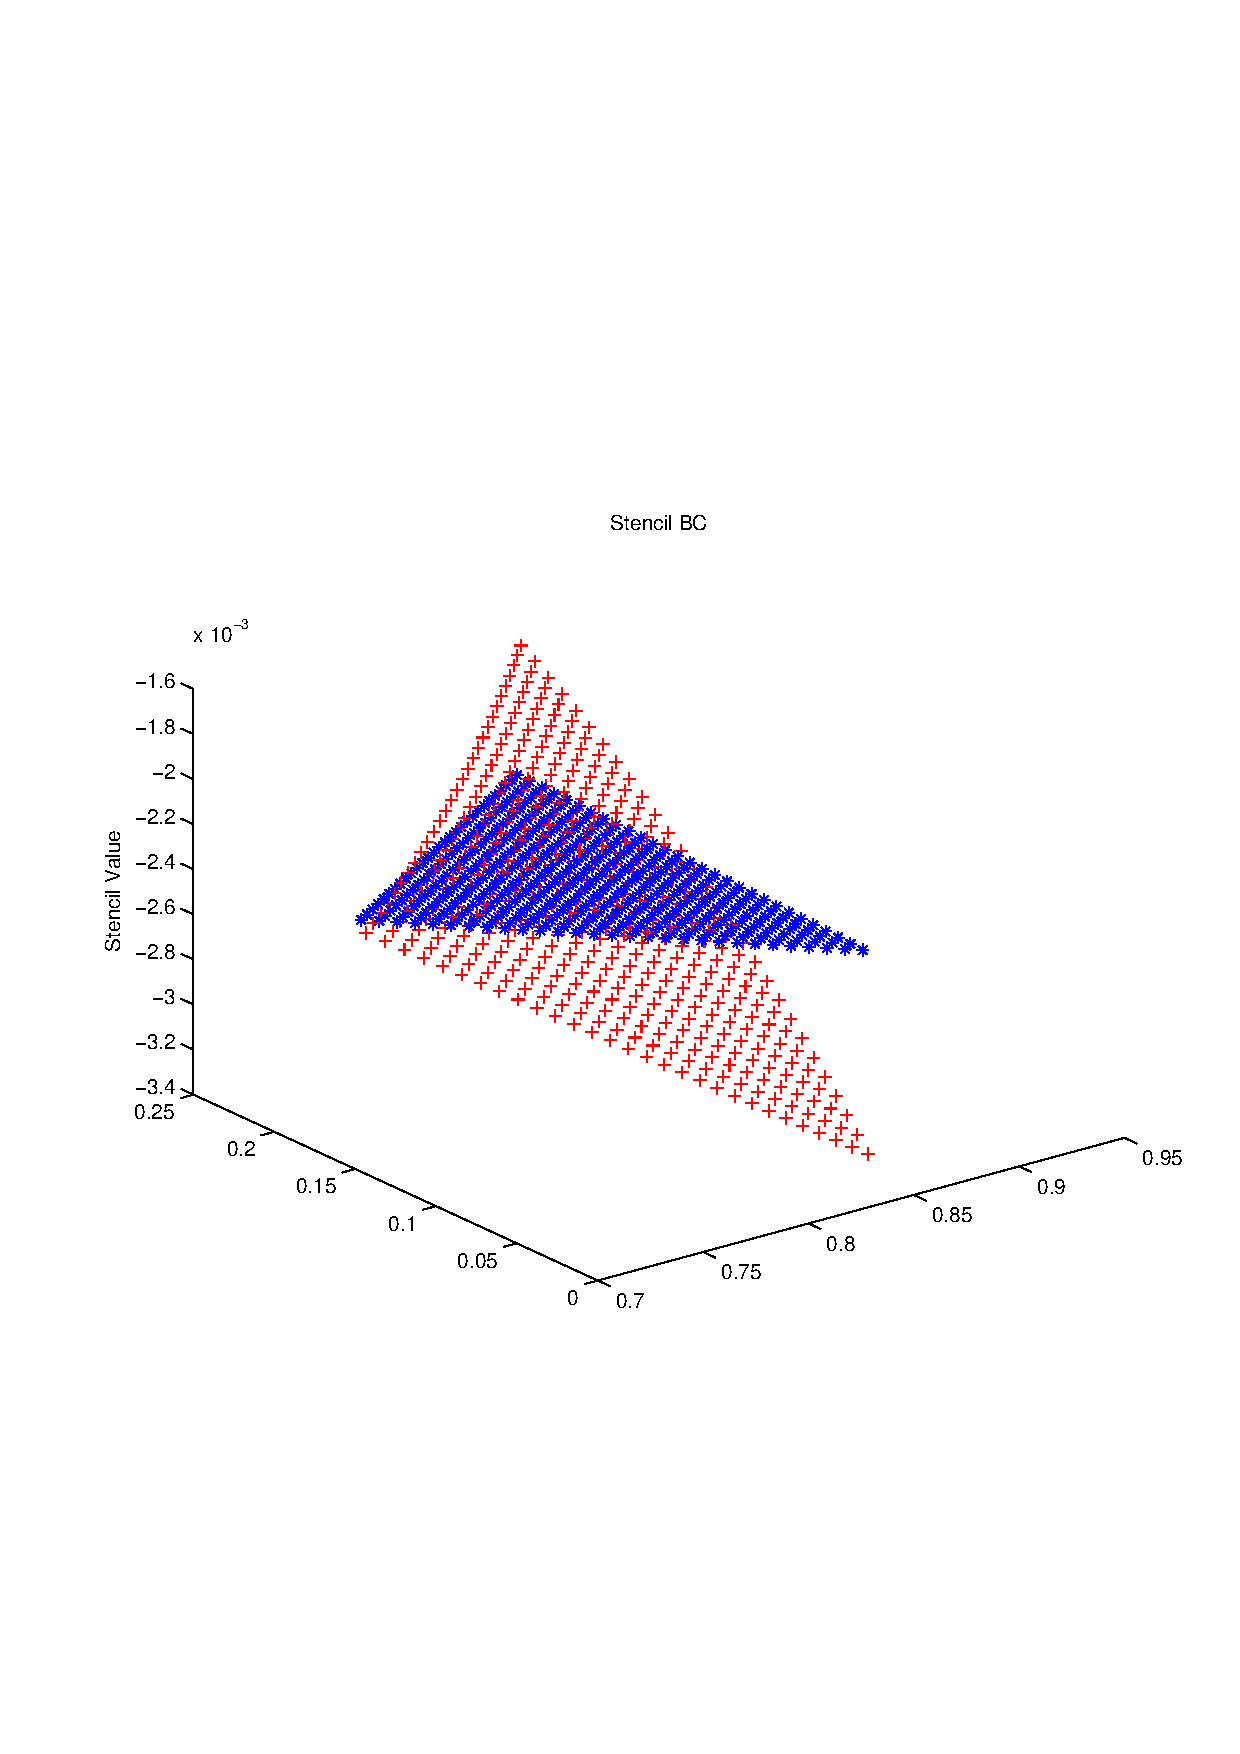
\includegraphics[width=0.98\textwidth]{stencilBC_nE}\\
  Stencil Entry BC
\end{column}\hfill
\begin{column}[T]{4.1cm} 
  \centering
  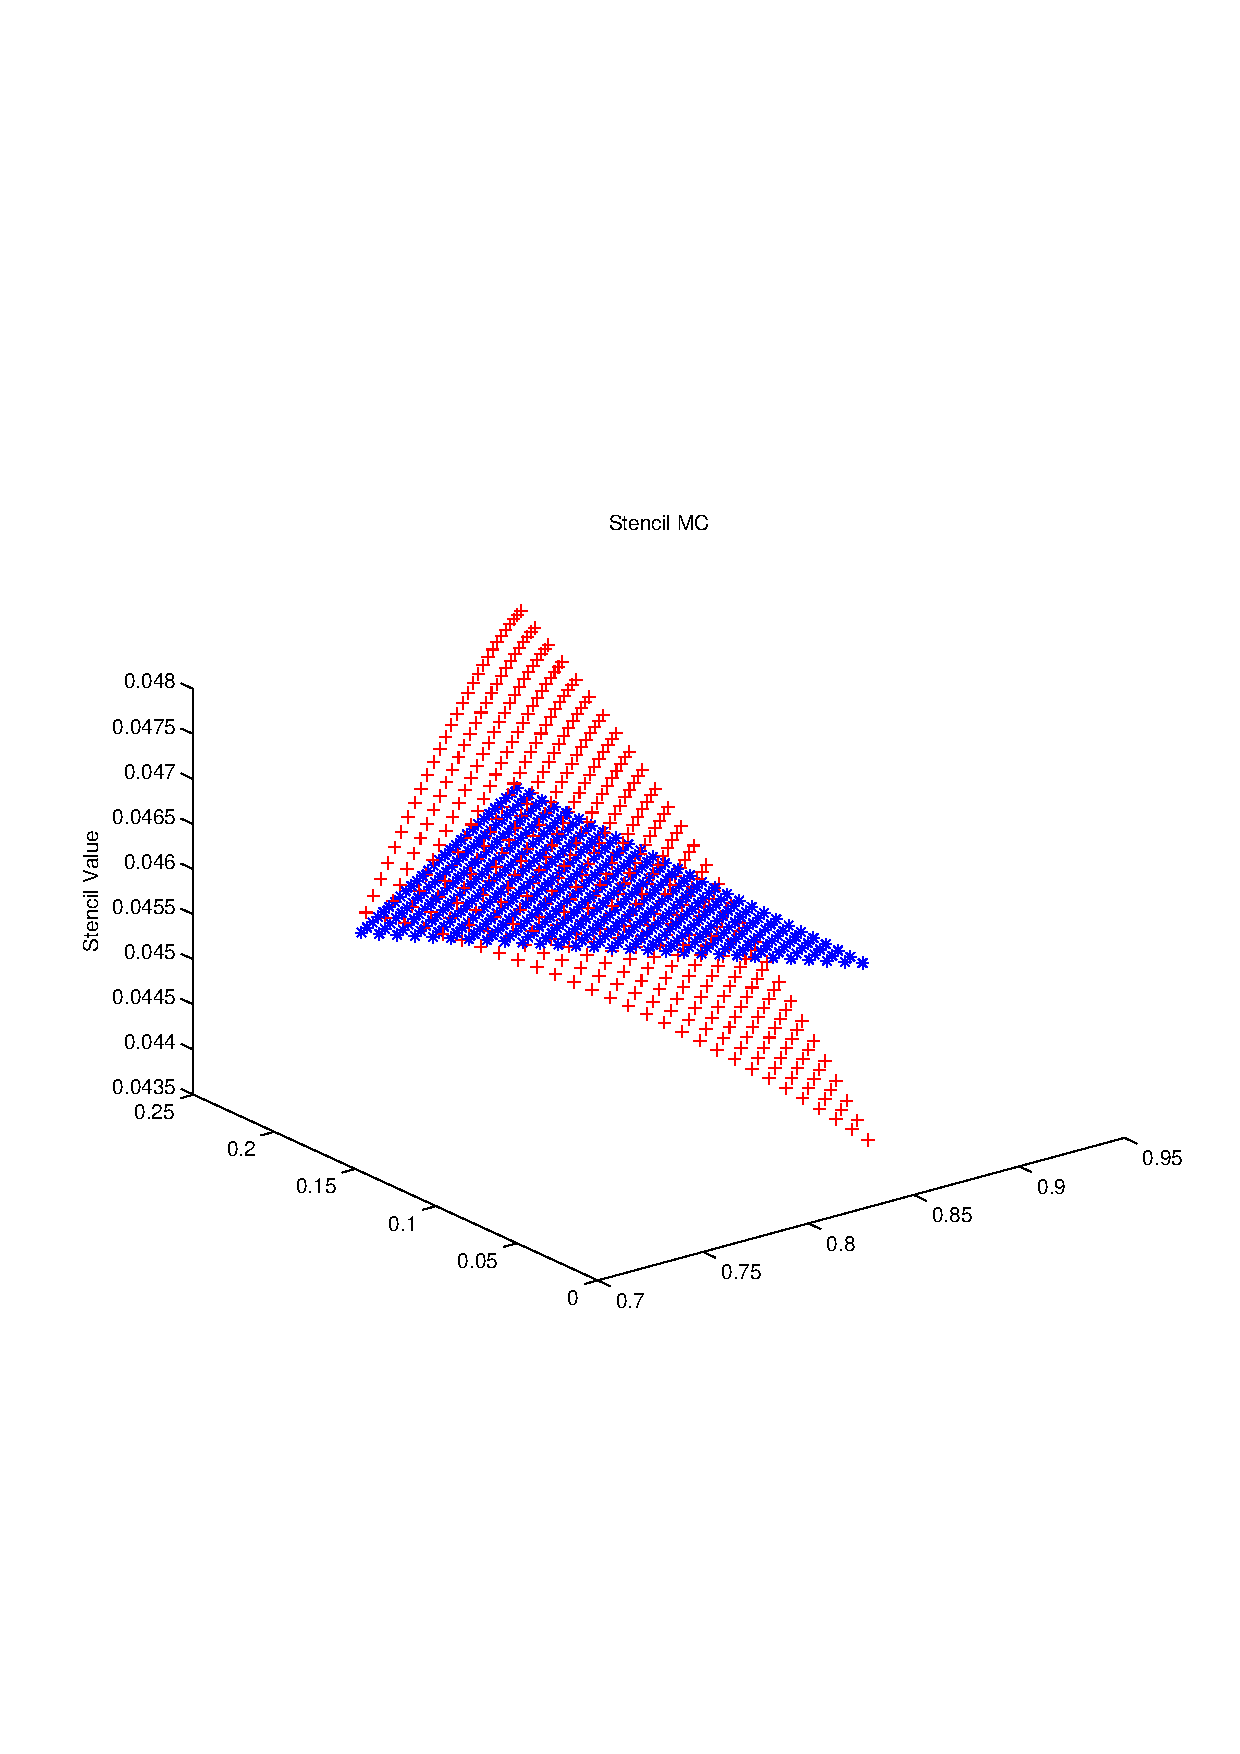
\includegraphics[width=0.98\textwidth]{stencilMC_nE}\\
  Stencil Entry MC
\end{column}\hfill
\begin{column}[T]{4.1cm} 
  \centering
  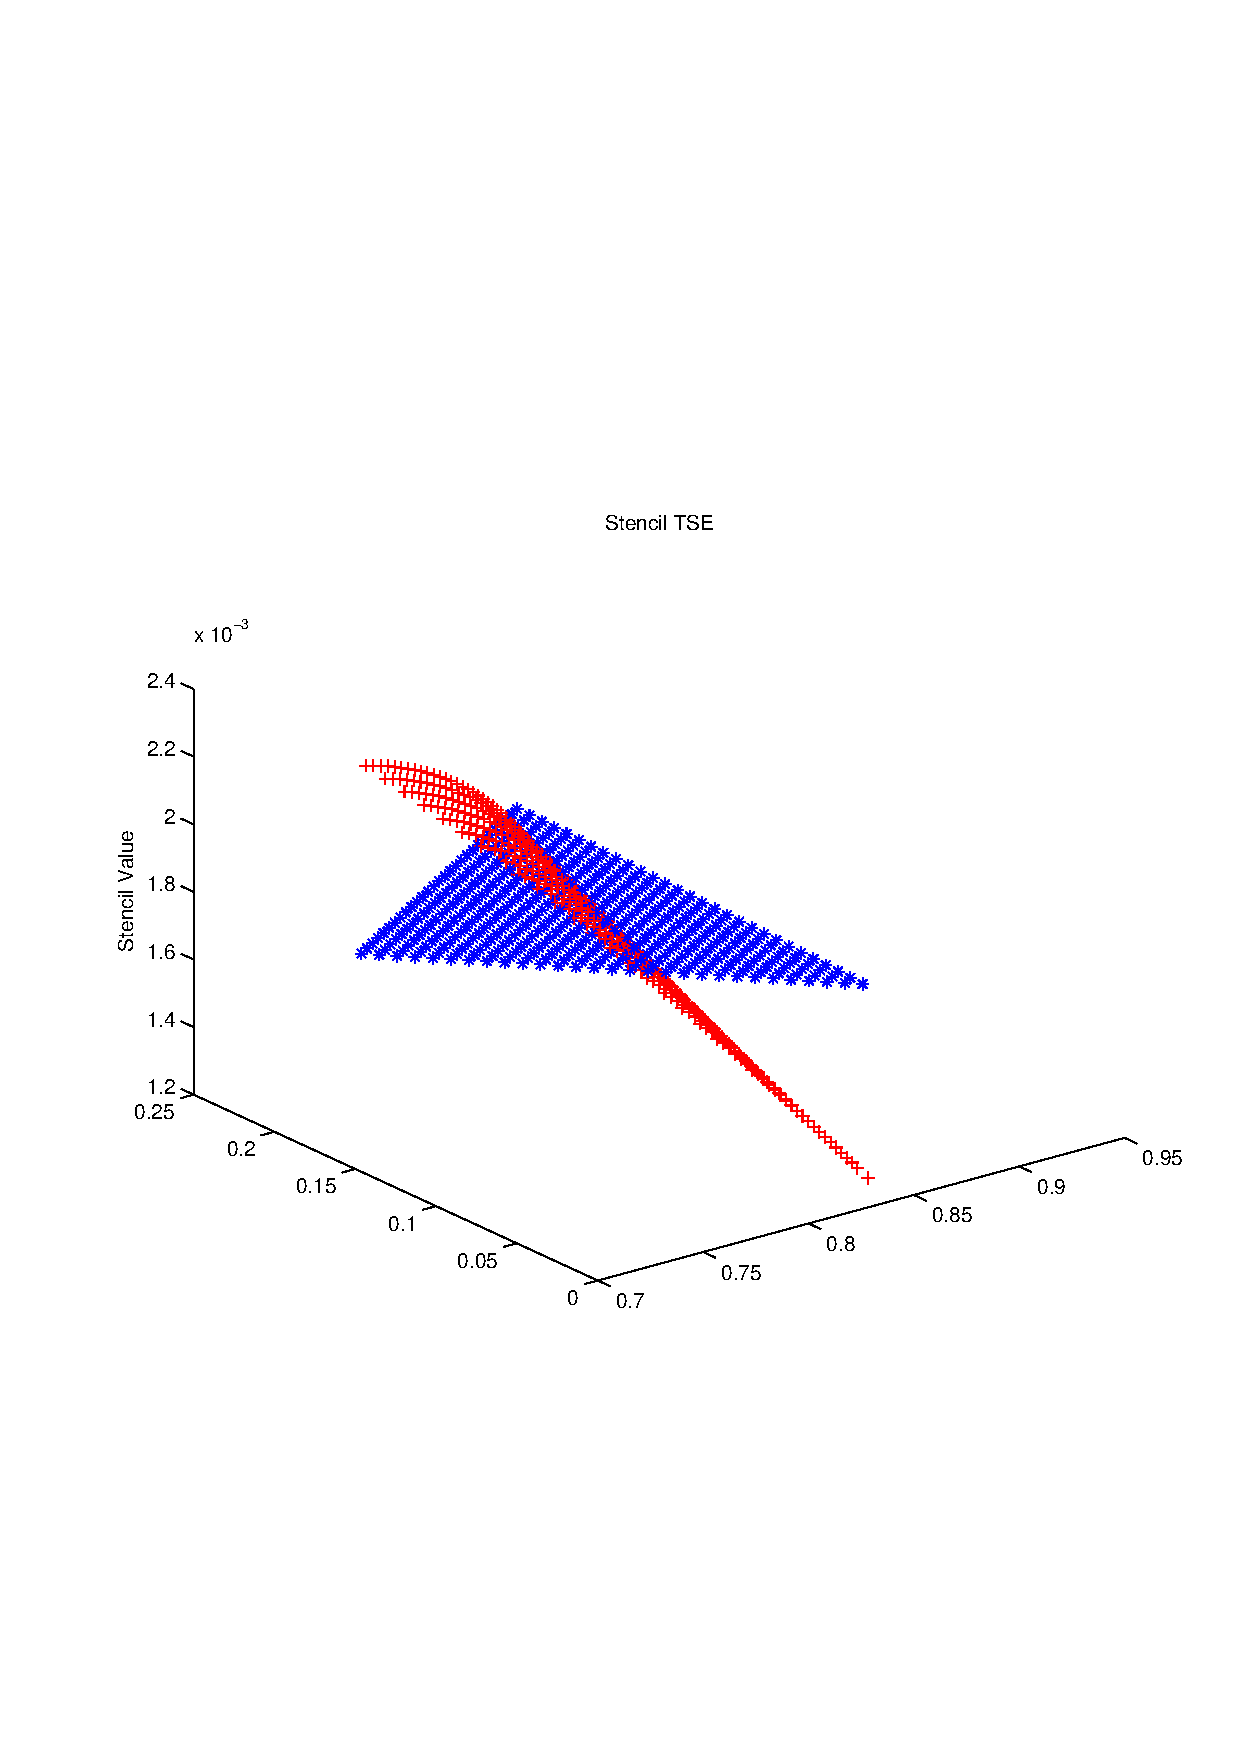
\includegraphics[width=0.98\textwidth]{stencilTSE_nE}\\
  Stencil Entry TSE
\end{column}
\end{columns}
\vspace{0.5cm}
\centering
Constant (blue) and projecte% =============================================================================
%    Results for spherepoisson
% =============================================================================
%
\section{Spherepoisson}
\subsection{Spherepoisson}d (red) stencil entries for all nodes of one plane
within one macro tetrahedron at refinement level 5


\end{frame}

%
% =============================================================================
%
\begin{frame}\frametitle{Stencils - Interpolation}


\rBox{Observation:} The displacements of the projected stencils exhibt
a smooth shape with some curvature.\\
\vspace{4ex}
\yBox{How can we utilize this?}\\
\vspace{4ex} 
\oBox{Idea:} Explicitly compute stencils only at some predefined sample
points and perform interpolation for all other points 

Questions: 
\begin{itemize}
\item{Which polynomial degree?}
\item{How much speed up can we gain?}
\item{Is this modified system still consistent with the original problem? }
\end{itemize}



\end{frame}

%
% =============================================================================
%
\begin{frame}\frametitle{Stencils - Interpolation }

\begin{itemize}
\item{linear    $\rightarrow$ not suitable due to the curvature}
\item{\oBox{quadratic} $\rightarrow$ resolves (moderate) curvature}
\item{cubic     $\rightarrow$ resolves curvature, but gets expensive}
\end{itemize}

\begin{figure}[htbp]
  \begin{minipage}{0.48\textwidth}   
For (tri-)quadratic interpolation we need 10 sample points.
This leads to the ansatz function:  
\begin{align*}
\label{eq:quadraticPolynomial}
a_{200}x^2 &+ a_{020}y^2 + a_{002}z^2 \\
+ a_{110}xy &+ a_{101}xz + a_{011}yz \\
+ a_{100}x &+ a_{010}y + a_{001}z \\
+ a_{000}
\end{align*}

  \end{minipage}
  \hfill
  \begin{minipage}{0.48\textwidth}
\includegraphics[width=0.98\textwidth]{tetSamplePointsPNG.png}
  \end{minipage}
\end{figure}


\end{frame}

%
% =============================================================================
%
\begin{frame}\frametitle{Interpolation - a first check}

\begin{columns}[T] 
\begin{column}[T]{4.1cm} 
  \centering
  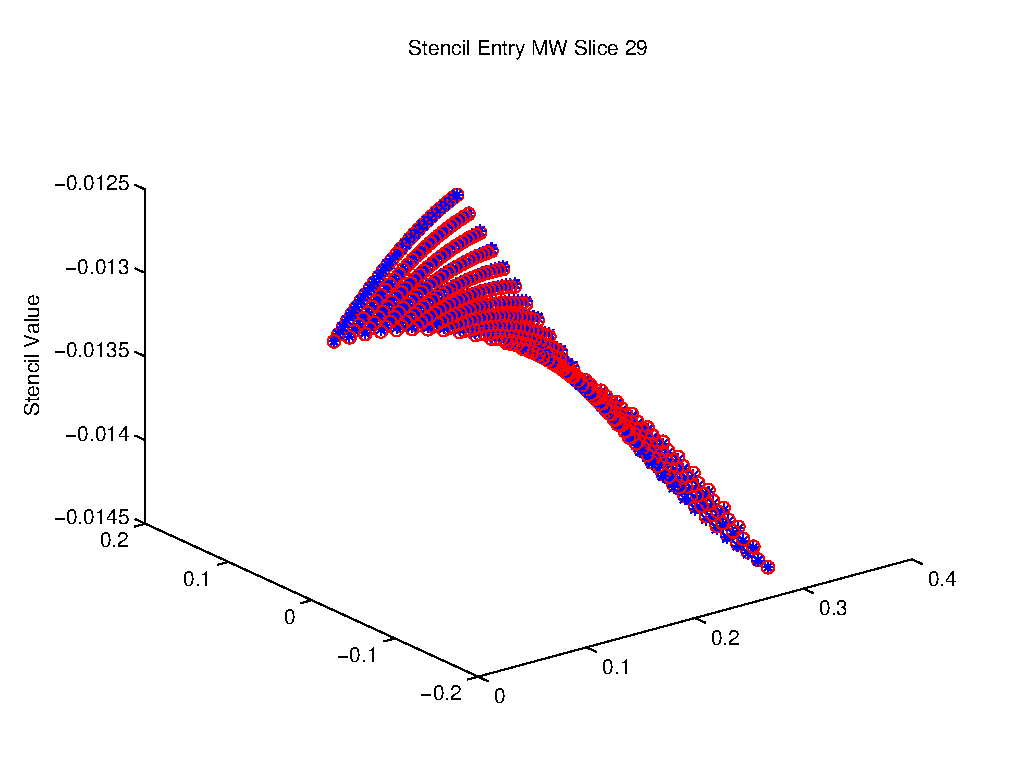
\includegraphics[width=0.98\textwidth]{stencilMW_slice29}\\
\end{column}\hfill
\begin{column}[T]{4.1cm} 
  \centering
  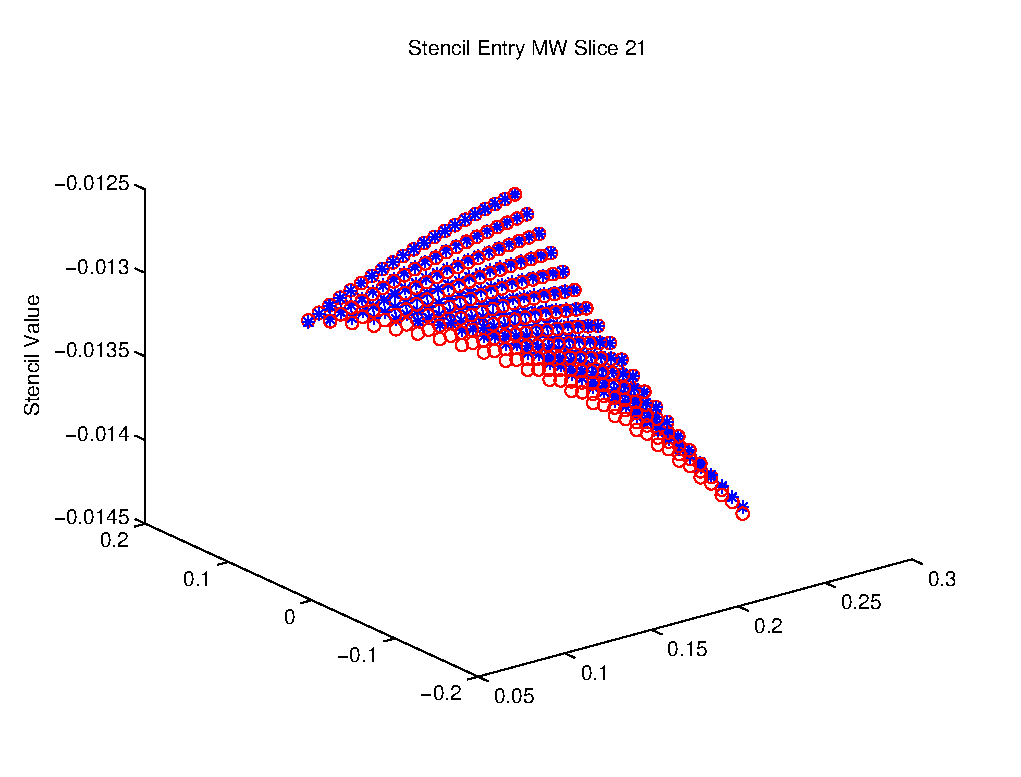
\includegraphics[width=0.98\textwidth]{stencilMW_slice21}\\
\end{column}\hfill
\begin{column}[T]{4.1cm} 
  \centering
  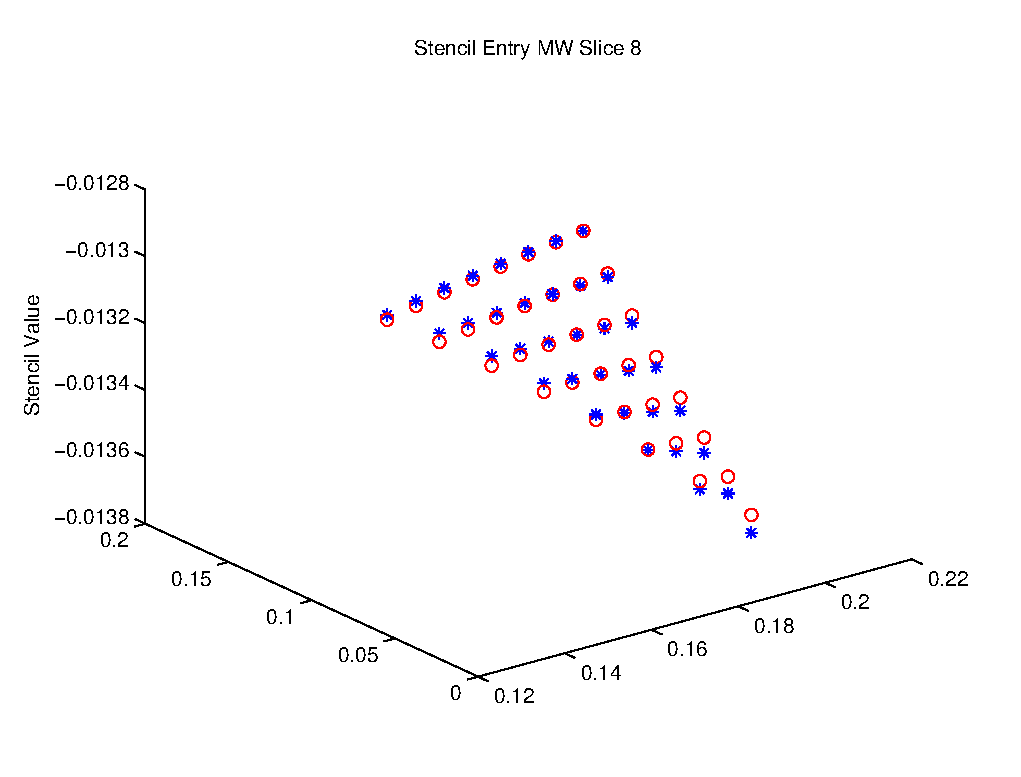
\includegraphics[width=0.98\textwidth]{stencilMW_slice8}\\
\end{column}
\end{columns}
\vspace{0.5cm}
\centering
Explicitly computed (projected) (blue dots) and interpolated 
(red circles) values for stencil entry
MW for different slices/planes within the macro tetrahedron
\end{frame}

%
% =============================================================================
%
\begin{frame}\frametitle{Interpolation of local stiffness matrices}


todo ...

\end{frame}

%
% =============================================================================
%
\begin{frame}\frametitle{Interpolation of local stiffness matrices}


\begin{theorem}
Both approaches are equivalent.
\end{theorem}

\begin{proof}
Schematically:\\
Employ the fact, that the functional
$\P_i : \RR^{10} \rightarrow \Pi^2$ which maps a
10-dimensional sample tuple 
onto a quadratic polynomial is \cempha{linear}.
Then, the order of stencil setup and interpolation 
can be reversed.
\end{proof}


\end{frame}

%
%
% =============================================================================
%
\begin{frame}\frametitle{HHG results - residual norm}

\begin{columns}[T] 
\begin{column}[T]{4.3cm} 
  \centering
  \includegraphics[width=0.98\textwidth]{spherepoisson_resEuc_level3}\\
  max. level 3
\end{column}\hfill
\begin{column}[T]{4.3cm} 
  \centering
  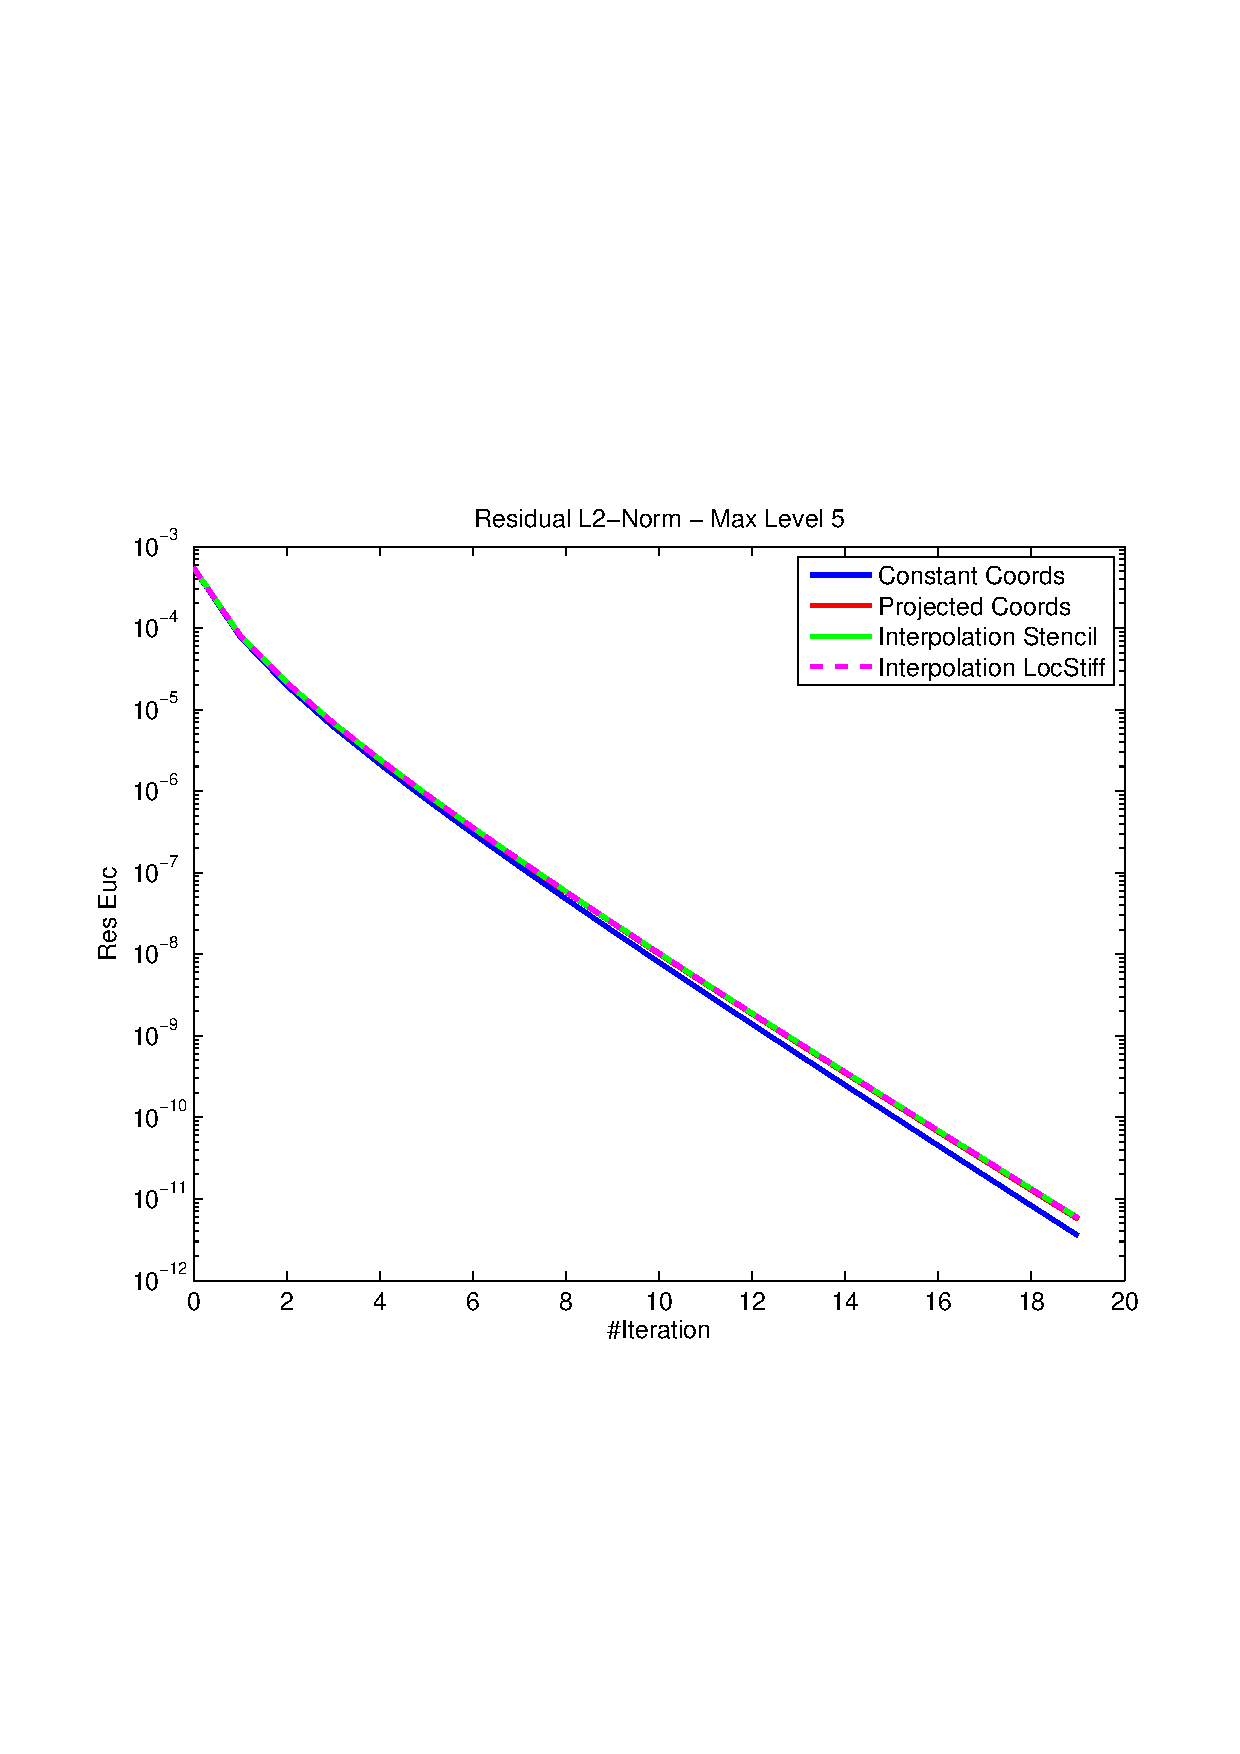
\includegraphics[width=0.98\textwidth]{spherepoisson_resEuc_level5}\\
  max. level 5
\end{column}\hfill
\begin{column}[T]{4.3cm} 
  \centering
  \includegraphics[width=0.98\textwidth]{spherepoisson_resEuc_level7}\\
  max. level 7
\end{column}
\end{columns}
\vspace{0.5cm}
\centering
Comparison of residual for constant (blue), projected (red), interpolated
stencil (green) and interpolated local stiffness matrices (magenta)
\end{frame}
%
%
% =============================================================================
%
\begin{frame}\frametitle{HHG results - CPU time}

\begin{columns}[T] 
\begin{column}[T]{4.3cm} 
  \centering
  \includegraphics[width=0.98\textwidth]{spherepoisson_cpuTime_level3}\\
  max. level 3
\end{column}\hfill
\begin{column}[T]{4.3cm} 
  \centering
  \includegraphics[width=0.98\textwidth]{spherepoisson_cpuTime_level5}\\
  max. level 5
\end{column}\hfill
\begin{column}[T]{4.3cm} 
  \centering
  \includegraphics[width=0.98\textwidth]{spherepoisson_cpuTime_level7}\\
  max. level 7
\end{column}
\end{columns}
\vspace{0.5cm}
\centering
Comparison of CPU time [sec] for constant (blue), projected (red), interpolated
stencil (green) and interpolated local stiffness matrices (magenta).
Jobs were done on borgcube with 32 procs.
\end{frame}

%
% =============================================================================
%
\begin{frame}\frametitle{HHG results - Discretization error}

\begin{columns}[T] 
\begin{column}[T]{4.3cm} 
  \centering
  \includegraphics[width=0.98\textwidth]{spherepoisson_errorEuc_level5}\\
  max. level 5
\end{column}\hfill
\begin{column}[T]{4.3cm} 
  \centering
  \includegraphics[width=0.98\textwidth]{spherepoisson_errorEuc_level6}\\
  max. level 6
\end{column}\hfill
\begin{column}[T]{4.3cm} 
  \centering
  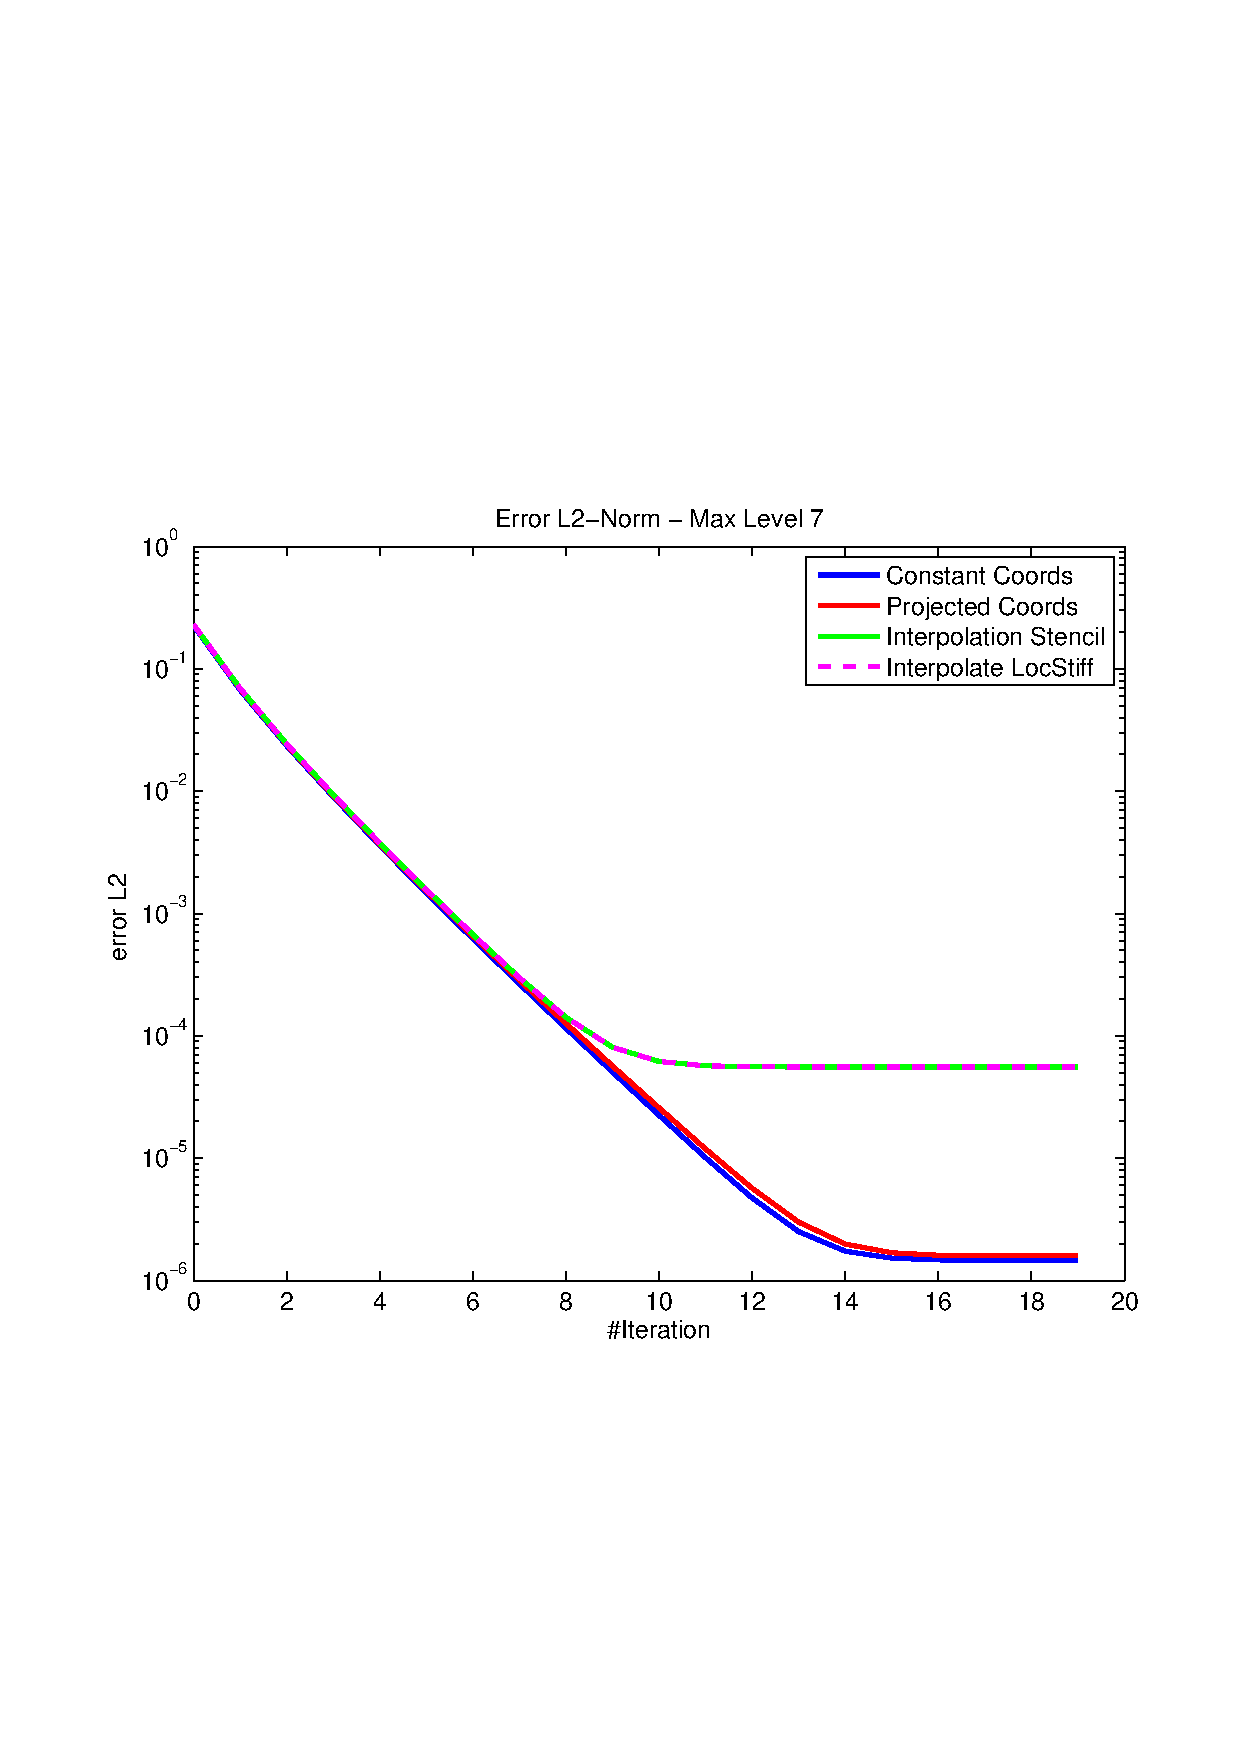
\includegraphics[width=0.98\textwidth]{spherepoisson_errorEuc_level7}\\
  max. level 7
\end{column}
\end{columns}
\vspace{0.5cm}
\centering
Comparison of discretization error for constant (blue), projected (red), interpolated
stencil (green) and interpolated local stiffness matrices (magenta).
Jobs were done on borgcube with 32 procs.
\end{frame}

%
% =============================================================================
%
\begin{frame}\frametitle{HHG results - Discretization error}

\begin{columns}[T] 
\begin{column}[T]{5.8cm} 
  \centering
  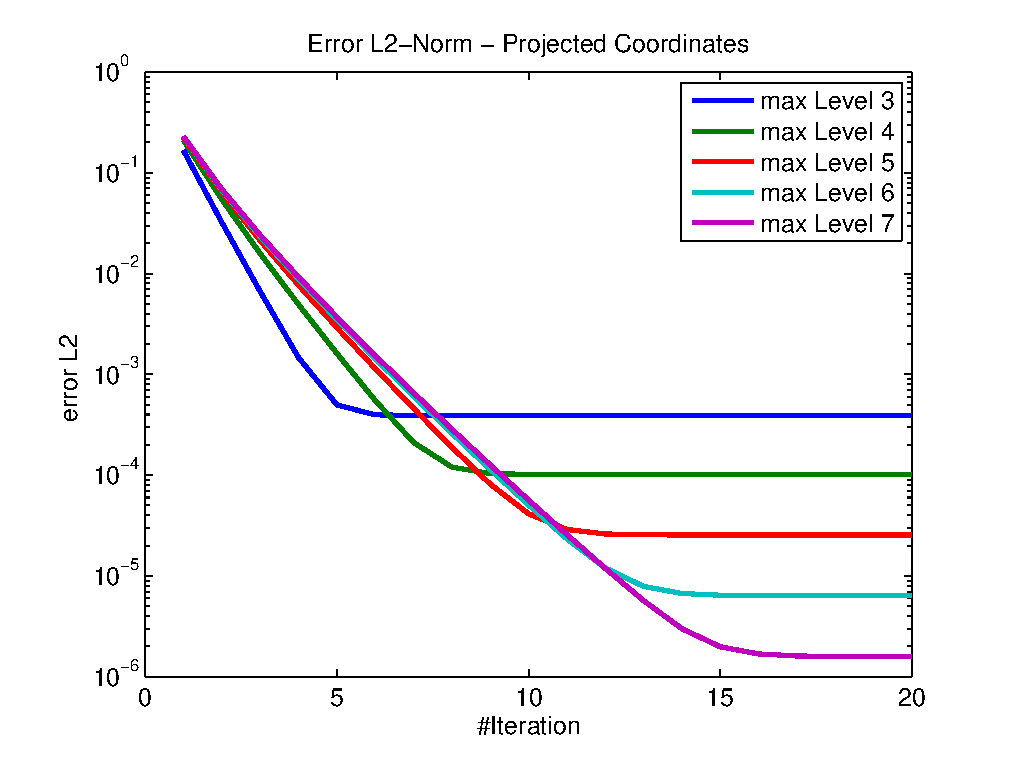
\includegraphics[width=0.98\textwidth]{spherepoisson_errorEuc_ProjCoords}\\
  projected coordinates
\end{column}\hfill
\begin{column}[T]{5.8cm} 
  \centering
  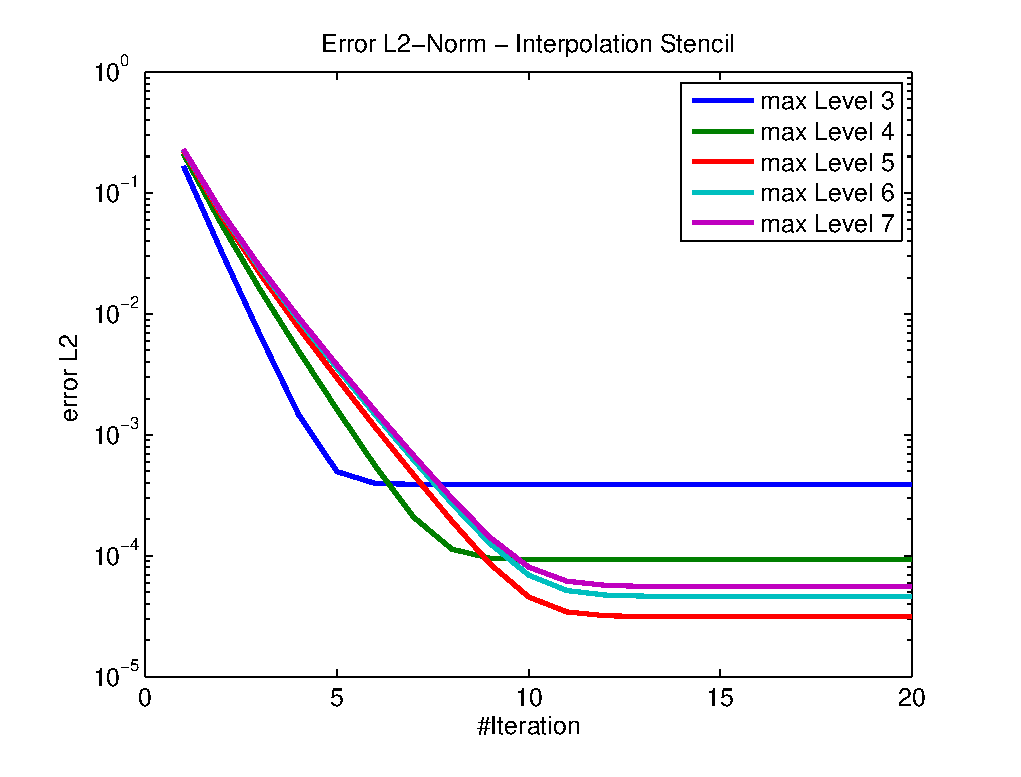
\includegraphics[width=0.98\textwidth]{spherepoisson_errorEuc_InterpolationStencil}\\
  interpolated stencils
\end{column}
\end{columns}
\vspace{0.5cm}
\centering

\end{frame}


% =============================================================================
%    Results for spherestokes
% =============================================================================
%
\section{Spherestokes}
\subsection{Spherestokes}
%
% =============================================================================
%
\begin{frame}\frametitle{HHG results - residual norm}

\begin{columns}[T] 
\begin{column}[T]{4.3cm} 
  \centering
  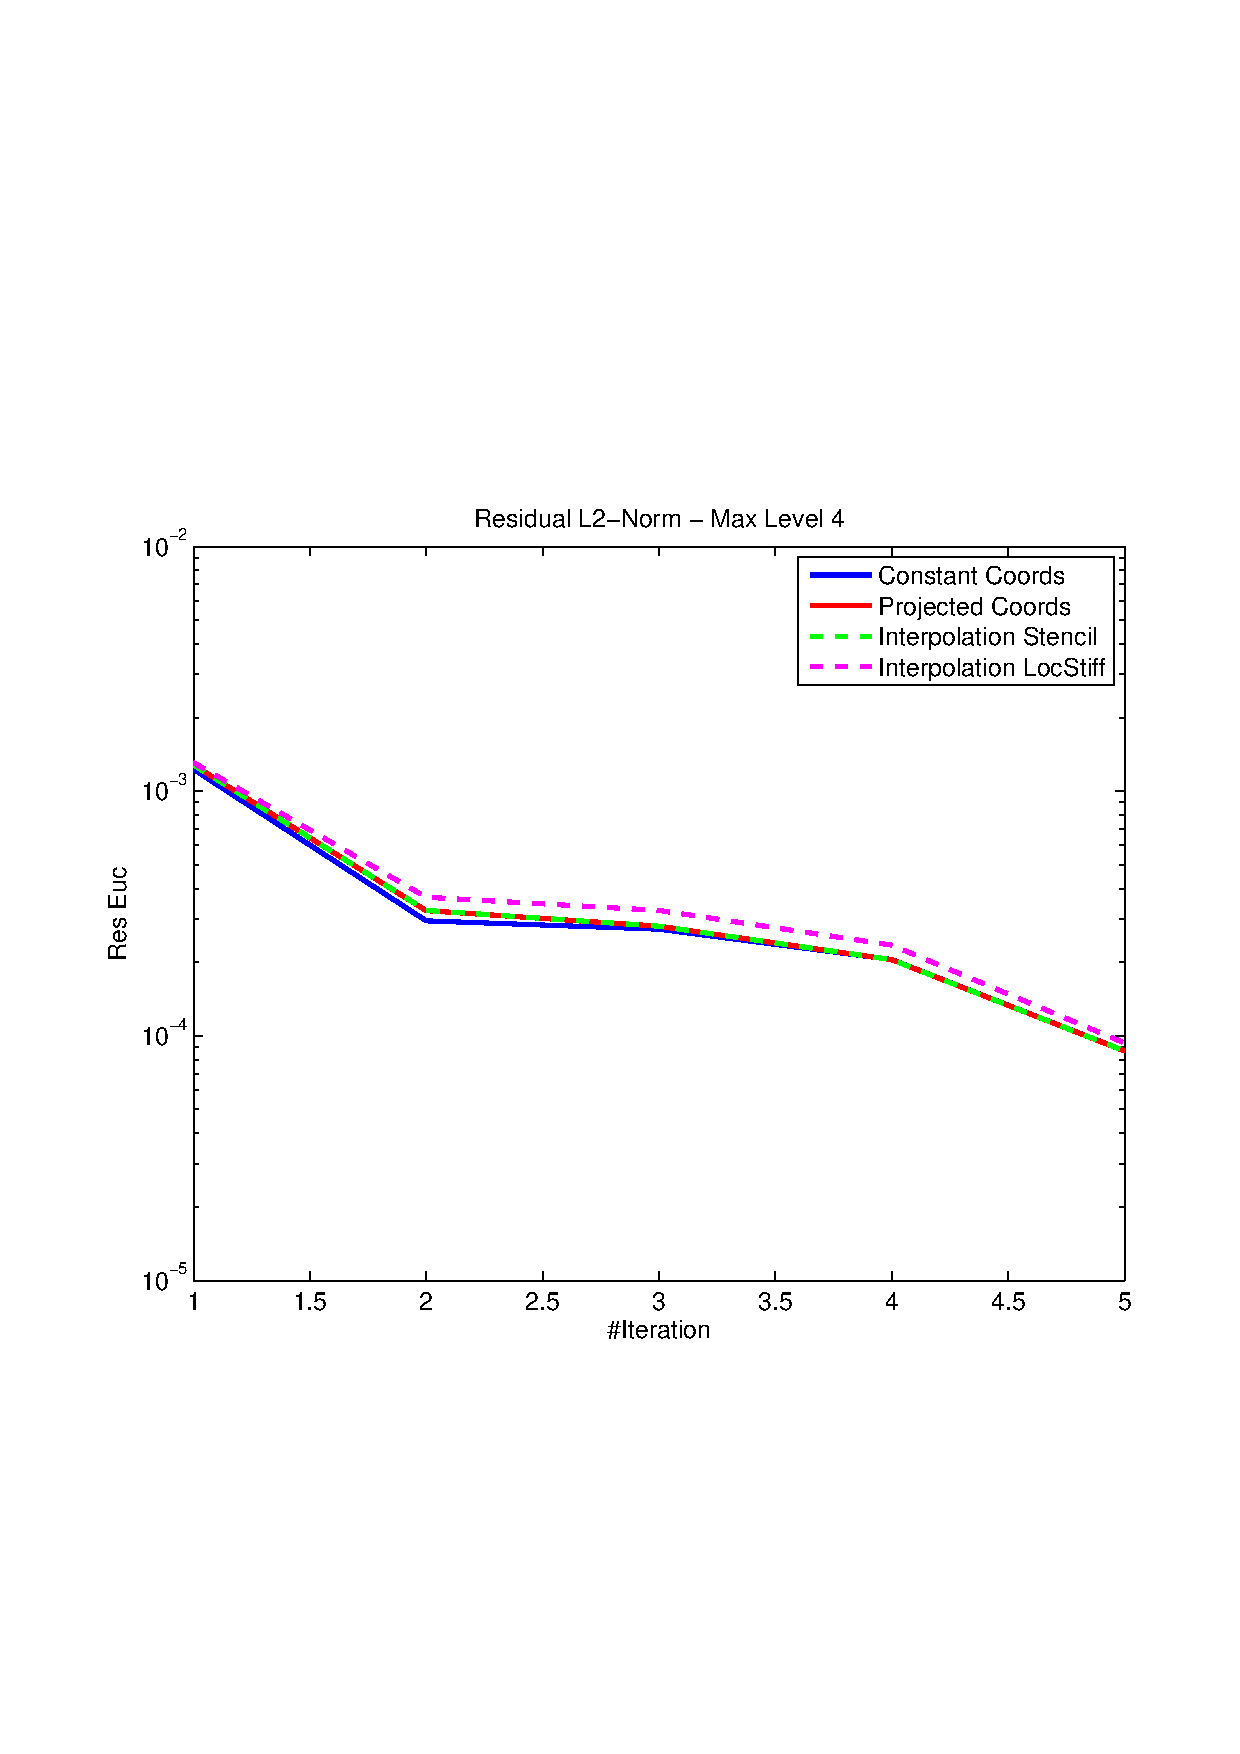
\includegraphics[width=0.98\textwidth]{spherestokes_resEuc_level4}\\
  max. level 4
\end{column}\hfill
\begin{column}[T]{4.3cm} 
  \centering
  \includegraphics[width=0.98\textwidth]{spherestokes_resEuc_level5}\\
  max. level 5
\end{column}\hfill
\begin{column}[T]{4.3cm} 
  \centering
  \includegraphics[width=0.98\textwidth]{spherestokes_resEuc_level6}\\
  max. level 6
\end{column}
\end{columns}
\vspace{0.5cm}
\centering
Comparison of residual for constant (blue), projected (red), interpolated
stencil (green) and interpolated local stiffness matrices (magenta)
\end{frame}
%
%
% =============================================================================
%
\begin{frame}\frametitle{HHG results - CPU time}

\begin{columns}[T] 
\begin{column}[T]{4.3cm} 
  \centering
  \includegraphics[width=0.98\textwidth]{spherestokes_cpuTime_level4}\\
  max. level 4
\end{column}\hfill
\begin{column}[T]{4.3cm} 
  \centering
  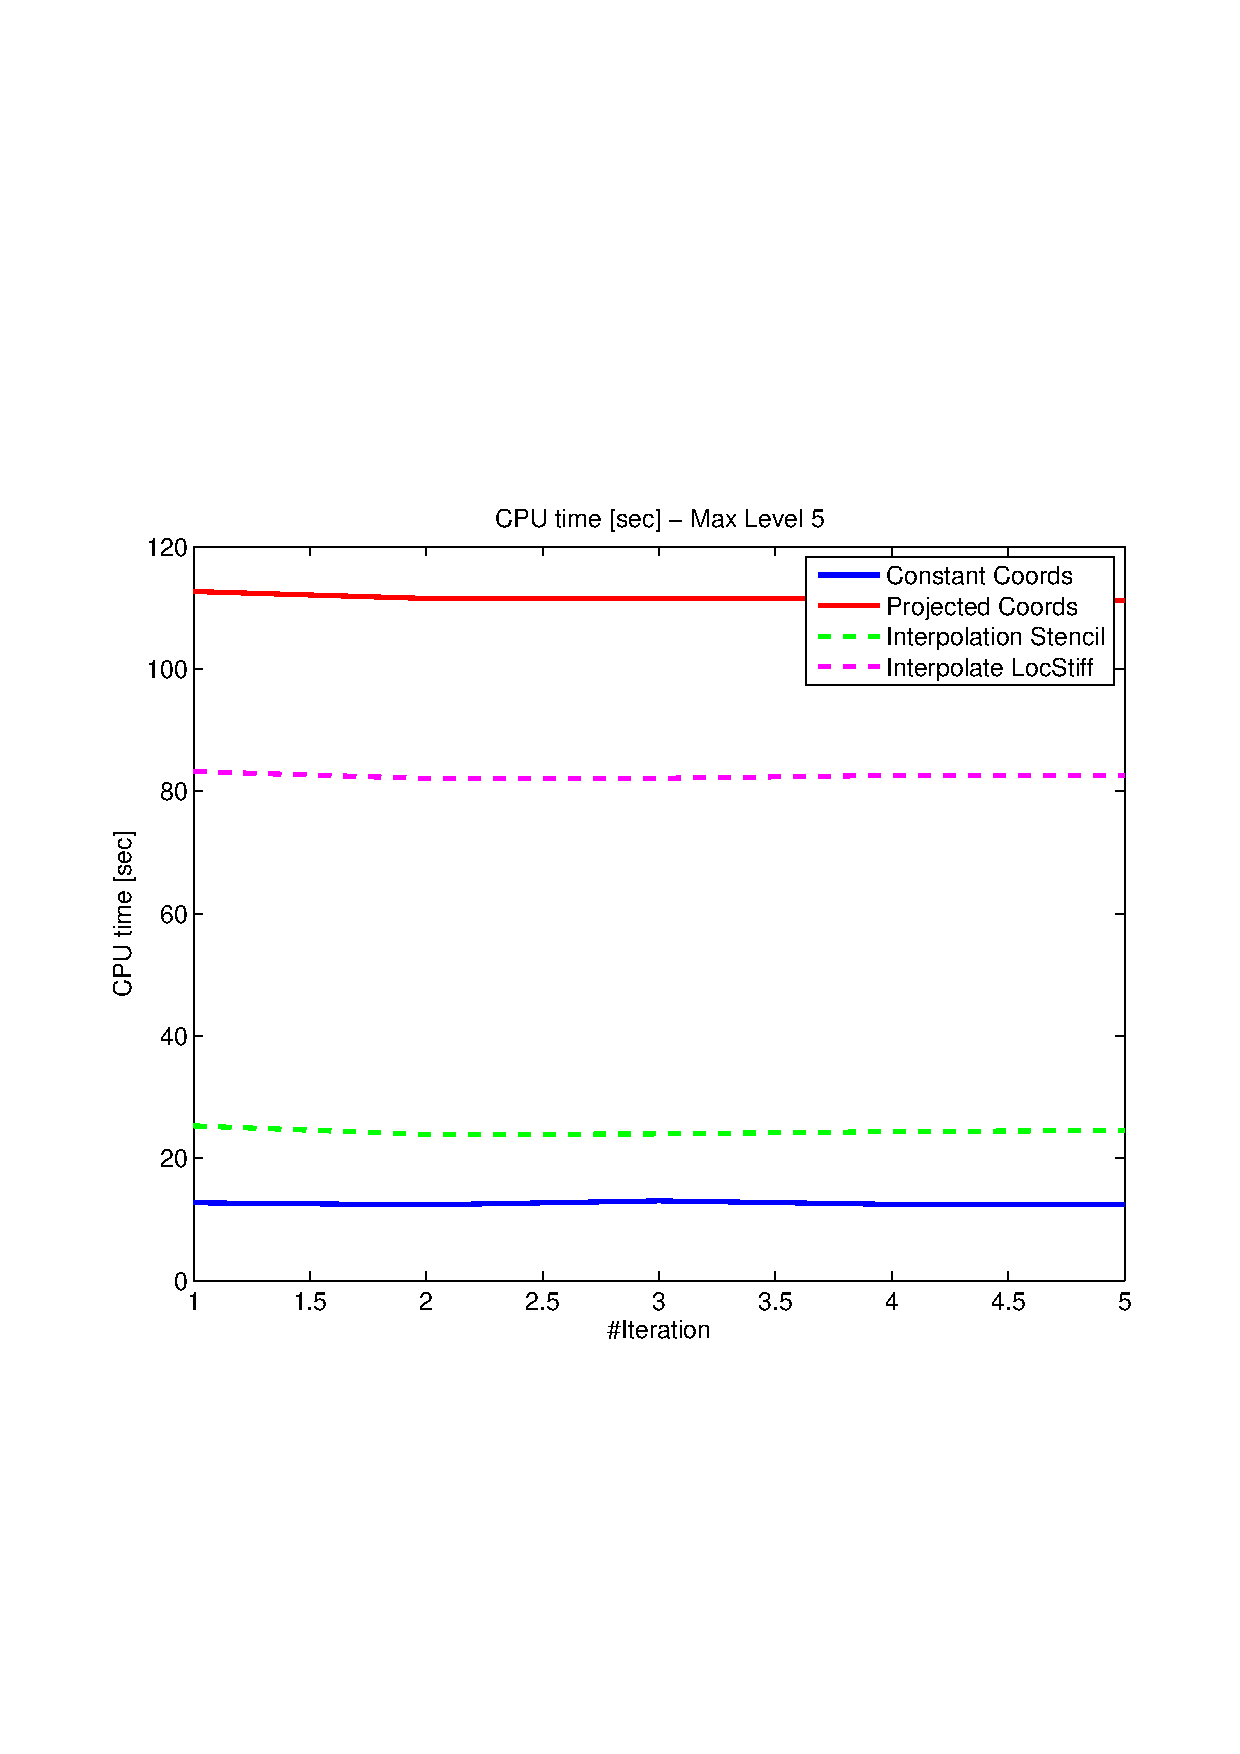
\includegraphics[width=0.98\textwidth]{spherestokes_cpuTime_level5}\\
  max. level 5
\end{column}\hfill
\begin{column}[T]{4.3cm} 
  \centering
  \includegraphics[width=0.98\textwidth]{spherestokes_cpuTime_level6}\\
  max. level 6
\end{column}
\end{columns}
\vspace{0.5cm}
\centering
Comparison of CPU time [sec] for constant (blue), projected (red), interpolated
stencil (green) and interpolated local stiffness matrices (magenta).
Jobs were done on borgcube with 32 procs.
\end{frame}

%
% =============================================================================
%
\begin{frame}\frametitle{HHG results - Discretization error}

\begin{columns}[T] 
\begin{column}[T]{4.3cm} 
  \centering
  \includegraphics[width=0.98\textwidth]{spherestokes_errorEuc_level4}\\
  max. level 4
\end{column}\hfill
\begin{column}[T]{4.3cm} 
  \centering
  \includegraphics[width=0.98\textwidth]{spherestokes_errorEuc_level5}\\
  max. level 5
\end{column}\hfill
\begin{column}[T]{4.3cm} 
  \centering
  \includegraphics[width=0.98\textwidth]{spherestokes_errorEuc_level6}\\
  max. level 6
\end{column}
\end{columns}
\vspace{0.5cm}
\centering
Comparison of discretization error for constant (blue), projected (red), interpolated
stencil (green) and interpolated local stiffness matrices (magenta).
Jobs were done on borgcube with 32 procs.
\end{frame}

% =============================================================================
%    Outlook
% =============================================================================
%
\section{Outlook}
\subsection{Outlook}
%
\begin{frame}\frametitle{Outlook}
%
todo...
%
\end{frame}
%
% =============================================================================
\end{document}
% =============================================================================
% EOF
% =============================================================================
